\documentclass[tikz,border=8pt]{standalone}
% Shared look for every TikZ diagram. Load with \input{../../tools/tikz-style.tex}
\usepackage[T1]{fontenc}
\usepackage{lmodern}
\renewcommand{\sfdefault}{lmr}  % diagrams use the same serif as the text
\usetikzlibrary{arrows.meta, positioning, shapes.geometric, calc, fit, backgrounds}
\definecolor{cblue}{HTML}{4C78A8}
\definecolor{corange}{HTML}{F58518}
\definecolor{cgreen}{HTML}{54A24B}
\definecolor{cred}{HTML}{E45756}
\definecolor{cpurple}{HTML}{B279A2}
\definecolor{cgrey}{HTML}{6B6B6B}
\tikzset{
  every picture/.style={font=\sffamily, line width=1.2pt},
  box/.style={draw=#1, fill=#1!12, rounded corners=4pt, align=center, inner sep=7pt, minimum height=1.1cm},
  box/.default=cgrey,
  arrow/.style={-{Stealth[length=3mm]}, draw=cgrey, line width=1.4pt},
  title/.style={font=\sffamily\bfseries\Large},
  note/.style={font=\sffamily\small, text=cgrey, align=center},
}
\AtBeginDocument{\hyphenpenalty=10000 \exhyphenpenalty=10000}

% The running example: a radio beacon on the wall 2 m to the side of the corridor at x = 6 m. The robot reads its
% straight-line distance h(x) = sqrt((6 - x)^2 + 2^2). Below: the curve h(x); x = 4 m and x = 8 m give the same 2.83 m.
\begin{document}
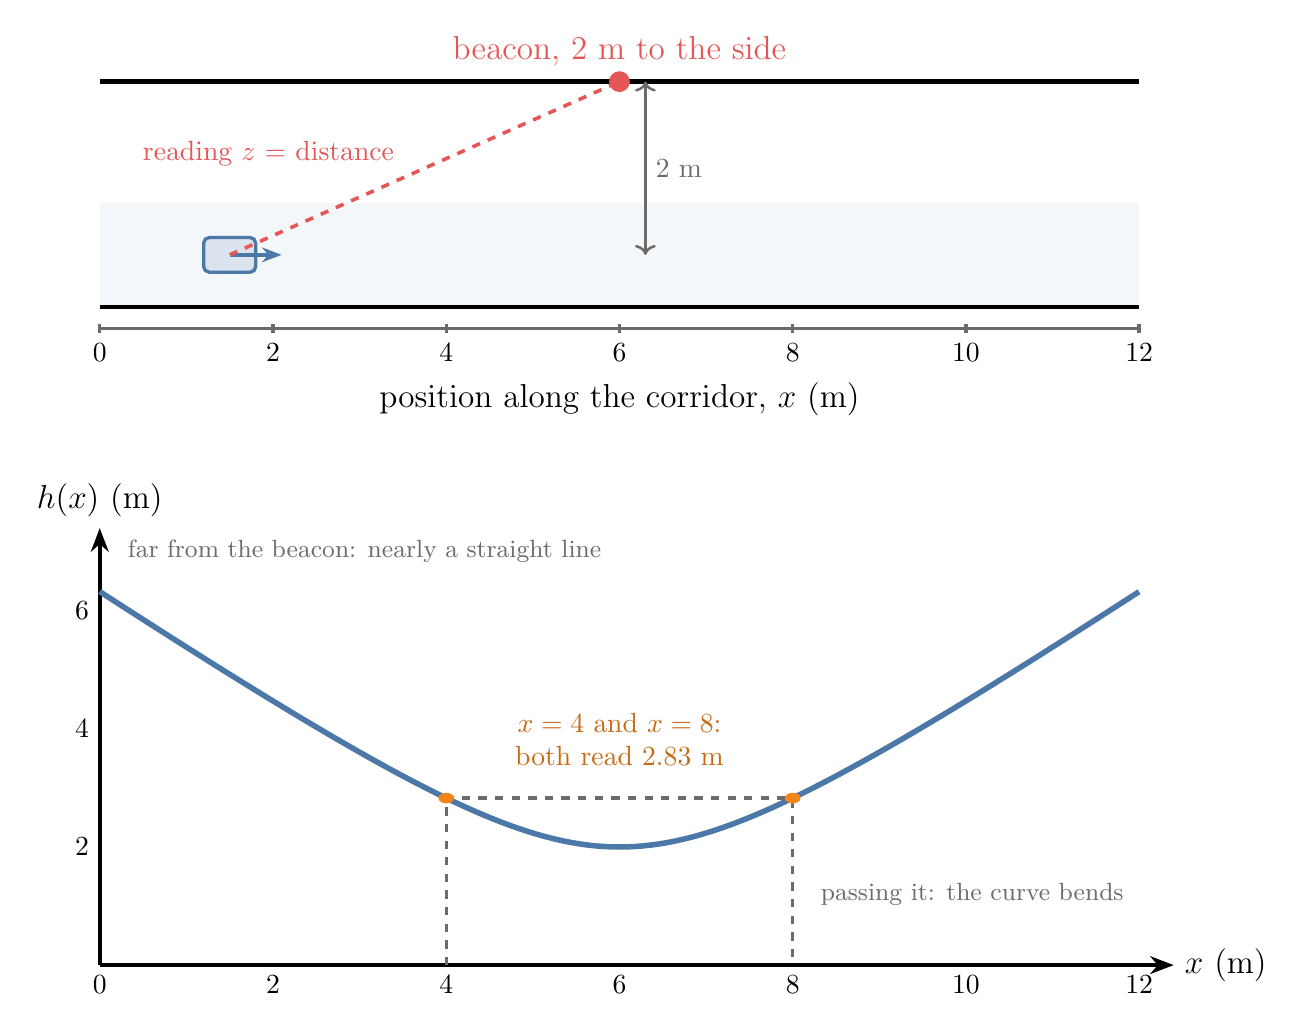
\begin{tikzpicture}[x=1.1cm, y=1.1cm, every node/.append style={font=\large}]
  % top view
  \fill[cblue!6] (0,0) rectangle (12,1.2);
  \draw[black, line width=1.6pt] (0,0) -- (12,0);
  \draw[black, line width=1.6pt] (0,2.6) -- (12,2.6);
  \fill[cred] (6,2.6) circle (0.12);
  \node[cred, above] at (6,2.65) {beacon, 2 m to the side};
  \begin{scope}[shift={(1.5,0.6)}]
    \draw[cblue, fill=cblue!20, rounded corners=2pt] (-0.3,-0.2) rectangle (0.3,0.2);
    \draw[-{Stealth[length=2.5mm]}, cblue, line width=1.6pt] (0,0) -- (0.6,0);
  \end{scope}
  \draw[cred, dashed, line width=1.3pt] (1.5,0.6) -- (6,2.6) node[pos=0.45, above left, font=\normalsize] {reading $z$ = distance};
  \draw[cgrey, <->, line width=0.9pt] (6.3,0.6) -- (6.3,2.6) node[midway, right, font=\normalsize] {2 m};
  \draw[cgrey, line width=0.8pt] (0,-0.25) -- (12,-0.25);
  \foreach \i in {0,2,...,12} {\draw[cgrey] (\i,-0.2) -- (\i,-0.3); \node[below, font=\normalsize] at (\i,-0.3) {\i};}
  \node[below] at (6,-0.75) {position along the corridor, $x$ (m)};
  % curve
  \begin{scope}[shift={(0,-7.6)}, y=0.75cm]
    \draw[arrow, draw=black] (0,0) -- (12.4,0) node[right] {$x$ (m)};
    \draw[arrow, draw=black] (0,0) -- (0,7.4) node[above] {$h(x)$ (m)};
    \draw[cblue, line width=2pt, domain=0:12, samples=120] plot (\x, {sqrt((6-\x)^2+4)});
    \foreach \i in {0,2,...,12} \node[below, font=\normalsize] at (\i,0) {\i};
    \foreach \j in {2,4,6} \node[left, font=\normalsize] at (0,\j) {\j};
    \draw[cgrey, dashed] (4,0) -- (4,2.828) -- (8,2.828) -- (8,0);
    \fill[corange] (4,2.828) circle (0.09) (8,2.828) circle (0.09);
    \node[corange!80!black, above, font=\normalsize, align=center] at (6,3.2) {$x = 4$ and $x = 8$:\\both read 2.83 m};
    \node[note, anchor=west] at (0.2,7.0) {far from the beacon: nearly a straight line};
    \node[note, anchor=west] at (8.2,1.2) {passing it: the curve bends};
  \end{scope}
\end{tikzpicture}
\end{document}
